\documentclass[11pt,letter]{article}
\usepackage[utf8]{inputenc}
\usepackage{amsmath}
\usepackage{amsfonts}
\usepackage{amssymb}
\usepackage{graphicx}
\usepackage[pdfborder={0 0 0},colorlinks=true,urlcolor=blue]{hyperref}
\usepackage{fullpage}
\usepackage{float}
\usepackage{textcomp}
\let\textquotedbl="
\usepackage{subscript}
\usepackage[T1]{fontenc}
\usepackage{subfig}
\usepackage{multirow}
\usepackage{pdfpages}

\newcommand{\scalefig}[3]{
  \begin{figure}[ht!]
    % Requires \usepackage{graphicx}
    \centering
    \includegraphics[width=#2\columnwidth]{#1}
    %%% I think \captionwidth (see above) can go away as long as
    %%% \centering is above
    %\captionwidth{#2\columnwidth}%
    \caption{#3}
    \label{#1}
  \end{figure}}

\begin{document}

\vspace*{3cm}
\begin{center}
{\bf 
{\fontsize{50cm}{25pt}\selectfont { Cubesat \\ \vspace{0.5cm} Literature Survey Report}} \\
\vspace{0.5cm}
{\large By}\\
\vspace{0.5cm}
{\Large Giri Subramanian (Student Researcher)\\
Rebecca Foust (Student Researcher)\\
Javier Navarro (Student Researcher)\\
David Hanley (Student Researcher)\\
Hong-Bin Yoon (Student Researcher)\\
Saptarshi Bandyopadhyay (Student Researcher)\\
Dan Morgan (Student Researcher)\\
Dr. Soon-Jo Chung (Principal Investigator)\\
Dr. Fred Y. Hadaegh (JPL Technical monitor)
}
}
\end{center}
\vspace{1cm}
\begin{figure}[!ht]
\centering
\subfloat{
\includegraphics[scale=0.5]{illinois_logo.png}} 
\hspace{2cm}
\subfloat{
\includegraphics[scale=0.5]{jpl_logo.jpg}}
\end{figure} 

\begin{center}
{{\bf \Large Department of Aerospace Engineering, \\
University of Illinois at Urbana-Champaign, \\ \vspace{0.2cm}
\today }}

\end{center}

\newpage
\begingroup
\hypersetup{linkcolor=black}
\tableofcontents
\listoffigures
\endgroup

\newpage
\section{Introduction}
In a world where lack of space is becoming an increasingly problematic issue to deal with, miniaturization is becoming more of  a necessity rather than an option. With sensors and actuators reaching really small scales, it is now possible to actually design pico and nano satellites to meet certain required scientific goals. In this report, we are majorly concerned with nano satellites or \href{http://www.cubesat.org/images/developers/cds_rev12.pdf}{CubeSats} with sizes ranging from 1U(10cm x 10cm x 10cm) to 6U(60cm x 10cm x 10cm). Since Cubesats are small, it is possible to launch multiple Cubesats with a single scientific mission. Thus using formation flying Cubesats it is possible to perform missions which, earlier, were either too difficult to do or required much bigger satellites. \\

The objective of this literature survey is three-fold: 
\begin{enumerate}
\item To find out and understand the existing single, as well as multiple, satellite missions and some proposed concepts.
\item To find out the various actuators and sensors that are available today or will be available in the near future (with an acceptable Technology Readiness Level) and to analyse if they would satisfy our mission requirements. 
\item To propose new missions based on formation flying of CubeSats.
\end{enumerate}


These missions have been categorized into four different classes as \href{http://solarsystem.nasa.gov/multimedia/download-detail.cfm?DL_ID=742}{Planetary Science}, \href{http://www.nap.edu/catalog.php?record_id=11820}{Earth Science}, \href{http://www.nap.edu/catalog.php?record_id=12951}{Astrophysics} and \href{http://www.nap.edu/catalog.php?record_id=13060}{Heliophysics}. There is also two charts presented at the end of these four sections, which give an idea of the various concepts that can be realized along with their scientific requirements. 

\section{Earth Science Missions}

\subsection{Cubesat investigating Atmospheric Density Response to Extreme driving (CADRE)}
This project's  main instrument is a 3-Unit (3U) CubeSat which is named as Cubesat investigating Atmospheric Density Response to Extreme driving (CADRE). The major issues addressed are related to ion-neutral coupling, which includes neutral wind morphology and dynamics which are very important for understanding how the thermosphere reacts to energy input and the role this plays in magnetosphere-ionosphere coupling. This is currently being carried out by Aaron Ridley at University of Michigan. \href{http://nsf.gov/awardsearch/showAward?AWD_ID=1042815&HistoricalAwards=false}{The link to the NSF award.}

\subsection{Collaborative Research: CubeSat--Composition Variations in the Exosphere, Thermosphere, and Topside Ionosphere (EXOCUBE)}

This project measures the densities of all significant neutral and ionized species in the upper atmosphere on a global scale. It is a 3U CubeSat. The main objective of this project is to provide the first in-situ global neutral density data in more than 25 years, which includes using the mass spectrometer technique to directly measure Hydrogen densities. This missions also provides observational constraints for physical models of the upper atmosphere. Also, newly developed experimental techniques which are used to obtain neutral and ionized composition and densities from radar and optical observations can be tested and validated using the measurements from this mission. This is currently being done by John Noto at Scientific Solutions Incorporated. \href{http://nsf.gov/awardsearch/showAward?AWD_ID=1042837&HistoricalAwards=false}{The link to the NSF award.}



\subsection{Ionosphere Monitoring}

\subsubsection{Predicting Earthquakes through Ionosphere Monitoring}

Early earthquake detection could help the third of a population that
is affected by earthquakes. Precursors to the earthquake can be detected
through variations in the ionosphere. The proposed satellite will
have a RAS topside sounder and be used to monitor the areas of the
Earth that have high seismic activity to predict earthquakes and prove
that the prediction method is valid and accurate. The data could also
help to improve GPS navigation models and study the reaction of the
ionosphere to magnetic events. The formation may help to mitigate
measurement errors.\cite{Ref:Jason} Something similar is scheduled
to be launched by the Chinese in 2014, though not a formation\cite{Ref:Earthquake}. 


\subsubsection{Studying the Reaction of the Ionosphere to Storms }

Magnetic storms can cause changes and bulges in the ionosphere. Understanding
these bulges can help us to understand the magnetic storm that causes
them as well. The DICE mission has studied this using 2 satellites
equipped with langmuir and electric field probes to measure the plasma
density and field strength. \cite{Ref:Crowley,Ref:Fish}

The ionospheric measurements can also track thunderstorms and cyclones
if positioned near the oxygen absorption line (\textasciitilde{}500
km) at a near-equatorial orbit using a microwave spectrometer. \cite{Ref:Blackwell}


\subsubsection{Monitoring Atmospheric Plasma Depletion to Predict Outages in GPS and Communications}

Depletion in ionospheric plasma can disrupt signal transferrance,
and not much is known about the depletion zones. The formation would
study how the depletions change and propagate so that scientists can
create a model and further their understanding of the phenomenon.
The satellites would be in 360 km orbits at an inclination of 52 degrees
\cite{Ref:Krause}\cite{Ref:Bracikowski}. These measurements can
also help to show the interactions between the thermosphere and ionosphere
\cite{Ref:Blalthazor}.

\subsection{Earth Imaging for Science Applications in Emerging Countries}

A satellite imaging cluster would give less advanced parts of the
world access to scientific data on things like resource consumption,
pollution, and climate. The formation could do the imaging with each
satellite operating a different camera type. The placement can range
from 400-720 km, but the effects of the high drag environment make
control much more difficult\cite{Ref:Harrison} \cite{Ref:Atir} \cite{Ref:Herscovitz}\cite{Ref:Kalman}\cite{Ref:Kim}.

The Nigerian government is launching a satellite of this type to monitor
environmental issues within the country, provide high volume mapping
data, and highly accurate image targeting and geolocation\cite{Ref:Curiel}. 

\subsection{Observing Gamma Rays Emitted by Thunderstorms}

The satellites will look for gamma rays emitted by thunderstorms in
visual and radio frequencies. NASA's Fermi telescope has observed
the phenomenon, but it could possibly do with more study and happen
in conjunction with the GRB monitoring.\cite{Ref:Fermi} \cite{Ref:Kitts}

\subsection{Space-Based Ocean Monitoring}

The health of Earth's bodies of water can be monitored through multi-spectral imaging with high spatial and temporal resolution. This will help scientists to better understand the effects of tides on ocean color, as well as the evolution of ecosystems. One study proposes using 115 nanosats for global coverage, but this is extremely ambitious, the formation would be much much smaller. \cite{Ref:Lowe}. The formation may not be able to add to the science.

\subsection{Testing Satellite Tether Deployment and Operations}

Satellite tethers can be used to create artificial gravity to aide
in long term human missions by tethering a crew module to an object
of equal mass and rotating the system. These systems need to be tested before they can be used for such operations. \cite{Ref:Carlson}\cite{Ref:Mazzoleni}

\subsection{Completing the Map of the Earth's Electric Field}

This project would use a system of small satellites to observe the
Earth's electric field with radar measurements. A proposed project
uses a constellation of 48 satellites. \cite{Ref:Redd}. Since it
is more appropriate for a constellation than for a formation, it is
not a great candidate for our project unless we wanted to create a
3D map. It would appear that other systems already make these measurements, but there are still areas of poor coverage that could be addressed \cite{Ref:ElecMap}. 

\subsection{Raman Spectroscopy to investigate the atmosphere}

Create a more in-depth model of the upper atmosphere using Raman Spectroscopy from multiple sources in a formation to achieve a 3D (or at least more comprehensive) map of planetary mineral and chemical abundances. The same technique could be used to study other planets as well \cite{Ref:Cantrell}. The main obstacle here would be finding a detector array that would fit in our size constraints. 

\subsection{Formation Flying to Sample Volume of Magnetosphere}

Use the formation of cubesats to create a more detailed 3D model of
the magnetosphere, adding detailed dynamic measurements. This may
not be necessary because of the twin satellites launched by NASA in
Fall 2012. Also several earlier missions acheived similar results,
not using formations but I doubt the information is still needed.\cite{Ref:Mag3D} In one proposed mission, a master satellite ejects several picosats which take 2-axis magnetometer data and relay it to the master. Relative position and attitude control are not necessary as long as the positions and attitudes can be discerned.\cite{Ref:Clarke}
\section{Planetary Science Missions}

\subsection{Mineral Mapping of Asteroids (Concept)}
The proposed mission overview is a single 6U CubeSat launched on a GEO satellite 
or Mars-bound mission as a secondary payload. There is a solar sail to reach near Earth asteroids. The proposed science objectives is to map surface composition of ~3 asteroids at 1-20 m spatial resolution.

Required instrumentation: ~spatial IFOV of 0.5 mrad, spatial sampling 0.5 m -10 m depending on the encounter range, Spectral sampling 10 nm, Imaging Spectrometer, 0.4 – 1.7 $\mu$m. Perhaps extend to 2.5 $\mu$m w/ HOT-BIRD or other advanced detector and achievable cooling. \href{http://kiss.caltech.edu/cosponsored/cubesat2012/presentations/staehle-interplanetary-cubesat-missions.pdf}{Link to presentation given by Robert Staehle}

\subsection{Solar system escape (Concept)}
The plan is to use a large area/ low mass spacecraft for high speed trajectory with low perihelion which would explore interplanetary environment, heliosheath and perhaps heliopause. It is also aimed to test communications, power, pointing and miniaturized instrument technologies.  \href{http://kiss.caltech.edu/cosponsored/cubesat2012/presentations/staehle-interplanetary-cubesat-missions.pdf}{Link to presentation given by Robert Staehle}

Required Instrumentation: Plasma, solar wind, Energetic particles \& cosmic rays, Magnetometer, Cameras to observe sail interaction with environment.


\subsection{Radio Quiet Lunar CubeSat (Concept)}
The aim is to assess radio quiet volume in shielded zone behind the Moon for future 21 cm cosmology missions. The proposed science mission is to find the usable volume behind the Moon for high sensitivity 21 cm cosmology observations which determines utility of lunar surface vs. orbiting missions.  \href{http://kiss.caltech.edu/cosponsored/cubesat2012/presentations/staehle-interplanetary-cubesat-missions.pdf}{Link to presentation given by Robert Staehle}

\subsection{Tracking Asteroids and Satellite Debris }

A formation of satellites would search for Earth-Approaching Asteroids
and potentially hazardous debris satellites using a small imaging
telescope \cite{Ref:Carroll}. One study suggests an orbit of 6000-40000
km \cite{Ref:Leitch}. 

Similarly, space debris of 1-10 cm is difficult to track using current
methods and can be very dangerous to things like solar arrays and
radiators \cite{Ref:Guerrero}. One study suggests the use of optical
and radar telescopes to track the small debris \cite{Ref:Tolkachev}.

\subsection{The CanX-4\&5 Formation Flying Mission: A Technology Pathfinder for Nanosatellite Constellations}

Accuracy and miniaturization of propulsion systems, attitude determination
sensors, control systems, inter-satellite communication systems and
relative position sensors is one of the key aspects for future small
satellite missions. The two spacecrafts Can X-4\&5 have been designed
as a technology demonstrator of these capabilities as independent
spacecraft but also to cooperate in flight formation. Both spacecrafts
will have access to the state vector of the other spacecraft wirelessly.
In addition, the pair of small satellite has been equipped with a
sub-meter relative position control, a centimeter-accuracy relative
position determination, a GPS receiver, an on board computer and an
inter-satellite communication system.\cite{Bonin_FF_CanX-4&5}

\subsection{Operations, Orbit Determination, and Formation Control of the AeroCube-4 CubeSats}

The company Aerospace Corporation built three satellites of the AeroCube-4
series that were launched in 2012. Each of these satellites was able
to estimate its position with 20m of accuracy by means of a GPS receiver
installed in each spacecraft. In addition, each satellite was equipped
with extendable wings that allowed variations in the cross-sectional
area of the spacecraft. This two features, the high precision orbital
positioning and the variable wings, allowed to measure the deliberate
changes in the drag profile caused by the different configurations
of the wing. The purpose of the project was to achieved formation
flight via wing manipulation and indeed the team succeeded reordering
the satellites over the course of several weeks.\cite{Gangestad_FF_AeroForces}

\subsection{Asteroid Prospector}

This paper contains the design of a small reusable spacecraft that
is able to go to asteroids from LEO as long as they are closer than
1.3 AU from the sun. The paper includes details on the several new
technologies that are needed to make this mission possible such as:
a 3 cm ion engine from Busek, the autonomous optical navigation system,
the precision miniature reaction wheels, and high performance green
propellant and Honeywell's new Dependable Multiprocessor.\cite{Muelle_AsteroidProspector}

\subsection{Real-Time Geolocation with a Satellite Formation}

This study demonstrates that a group of two or three satellites in
LEO is able to accurately position a source of electromagnetic pulses
on the surface of the Earth. The position of the emitting source is
computed using time difference of arriving signals. The study also
talks about how this could be beneficial for other missions such as
the Mars rover or a busy constellation of positioning satellites.\cite{Leiter_Geoloc}

\subsection{NASA\textquoteright{}s GRAIL Spacecraft Formation Flight, End of Mission Results, and Small-Satellite Applications}

This mission, the Gravity Recovery and Interior Laboratory (GRAIL),
consists of two identical spacecraft designed to map the variations
of the gravitational field of the Moon. To do so, it is of great importance
that the spacecrafts measure the distance in between with high accuracy
and also orbit in the same orbital plane and height over the Moon's
surface.\cite{Edward_GRAIL}

\section{Astrophysical Missions}

\subsection{Pinpointing the Source of Gamma Ray Bursts (Concept)}
\label{gamma_burst}

The formation could be used to source GRBs through precise triangulation. If researchers could receive the measurements of inter-satellite distance and GRB incident time accurately enough, they could potentially increase the accuracy of GRB detection and positioning. \cite{Ref:Dill}. This has since been proven unnecessary, there are sufficient satellites in orbit to do this, through the use of gamma ray detectors and UV detectors. The UV detectors can do the positioning that would have required a formation with only gamma ray detectors. 

\subsection{Interferometry and Synthetic Aperture Radar Formation Flying}
\label{sar}

A formation of >2 CubeSats will work together to create a digital
terrain model or study surface deformation. A cross-track pendulum
formation is easier to isolate the crosstrack and along-track components. A cartwheel formation, however, reduces the height errors \cite{Ref:Peterson}. The application is widely studied for formations. 

\subsection{Studying Sub-dwarf Stars Using a Small Telescope}
\label{dwarf}
A satellite-bourne telescope would be used to study distant sub-dwarf stars, to set the lower limit on the age of ``metal-poor sub-dwarf'' stars to help establish an age for the universe. The attitude control system would need to be accurate to within 30 arc-seconds \cite{Ref:Carroll2}. Another possible mission would be imaging star fields \cite{Ref:Nicholas}. To make the formation relevant, each satellite would need a different type of instrument to further the science. 

\subsection{Astronomical Antenna for a Space Based Low Frequency Radio Telescope}
\label{astro_ant}
A great atmospheric interference occurs for low radio frequencies,
specially bellow 30 MHz. For that reason low frequency radio telescopes
are not feasible on the surface of the Earth. Therefore the only way
to collect reliable data in that frequency is by placing the instruments
in space. The Orbiting Low Frequency Antennas for Radio Astronomy
(OLFAR) consists of a swarm of nano-satellites, each of them with
three dipoles that satisfy the space restrictions in cubesats, intended
to build a low-frequency distributed radio telescope in space. This
paper describes the design, simulations, testing and measurements
of a scale model of the system. \cite{Quillen_FF_RadioTelescope}

\subsection{PanelSAR: A Smallsat Radar Instrument}
\label{panelsar}
PanelSAR describes a solution to implement a low-cost and low power consuming synthetic aperture radar in a small satellite. The study states that a low power SAR, which has already been proved in aircraft, and several other features of the system, such as modularity, reliability and low mass are key to reach a low cost solution.\cite{Dujin_Radar}

\subsection{Deployable Mirror for Enhanced Imagery Suitable for Small Satellite Applications}
\label{deploy_mirror}

Small satellite volume restrictions are a clear drawback for large
aperture monolithic mirrors for telescopes. Consequently, high spatial
resolution can not be achieved with a single mirror. One solution
to this problem is the development of deployable optical systems that
could surpass the performance of monolithic mirrors and greatly improve
the capabilities of small satellites. A passively aligned deployable
mirror is under development by the Space Dynamics Laboratory (SDL) and
they have built one of the ``petals'' that conform the deployable
mirror. The spectrum they are interested in varies from short wave
infrared to long wave infrared due to the image quality obtained.\cite{Champagne_deployablemirror}

\subsection{Autonomous Assembly of a Reconfigurable Space Telescope (AAReST) \textendash{} A CubeSat/Microsatellite Based Technology Demonstrator}
\label{aarest}
This study has been reported here because it remarks the disadvantages
of formation flying satellites and proposes an alternative to formation
flight, namely autonomous assembly. The paper states that autonomous assembly
is cheaper and more efficient when building space telescopes with
large apertures. In addition, the study claims that it is difficult
to maintain a stable alignment among spacecrafts in flight formation.
The mission developed in the study contains two 3U cubesats, each
of them would operate an electrically actuated adaptive mirror. In
addition, there would be a central 9U cubesat core, housing two fixed
mirror, where the 3U cubesats could dock and un-dock.\cite{Underwood_ReconfigTelescope}
\section{Heliophysical Missions}

\subsection{Colorado Student Space Weather Experiment}
\label{colorado}

This is a three-year multi-disciplinary team effort and the aim is to and operate a CubeSat. This 3U Cubesat carries an energetic particle sensor which will address fundamental space weather science questions regarding topics like relationship between solar flares, energetic particles and geomagnetic storms in the near Earth space environment. The particle instrument is the Relativistic Electron and Proton Telescope integrated little experiment (REPTile). REPTile is designed to measure directional differential flux of energetic protons, 10-40 MeV, and electrons, 0.5 to $\textgreater$ 3 MeV.  The major science objectives of this project are to investigate the relationships between solar energetic particles, flares, and coronal mass ejections, and also to characterize the variations of the Earth's radiation belt electrons. This is currently being carried out by Xinlin Li at University of Colorado at Boulder. \href{http://nsf.gov/awardsearch/showAward?AWD_ID=1042815&HistoricalAwards=false}{The link to the NSF award.}

\subsection{Solar Polar Imager CubeSat Constellation (Concept)}
\label{solar_polar}
This mission is a concept of 6 spacecraft in a constellation of highly inclined orbits. They would be in an out-of-ecliptic vertical orbit. They will use solar sails to reach high inclination. The proposed science missions are include Helioseismology and studying the magnetic fields of polar regions, polar view of corona, coronal mass ejections, solar radiance and also to link high latitude solar wind \& energetic particles to coronal sources.  \href{http://kiss.caltech.edu/cosponsored/cubesat2012/presentations/staehle-interplanetary-cubesat-missions.pdf}{Link to presentation given by Robert Staehle}

The required instrumentation of the 6  satellites are:
\begin{itemize}
\item S/C1: Plasma + Mag Field 
\item S/C2: Energetic Particles + Mag Field 
\item S/C3: Cosmic Rays, 
\item S/C4: Magnetograph/Doppler Imager 
\item S/C5: EUV Imager 
\item S/C6: Coronagraph 
\end{itemize}


\subsection{Earth-Sun Sunward-of-L1 Solar Monitor (Concept)}
\label{l1}
The aim of this concept is to measure strong coronal mass ejections or other space weather from Sunward-of-L1 position to provide additional warning time to Earth. The science objective is to obtain plasma and magnetometer readings of solar wind from sunward-of-L1 position and to compare with L1 values from ACE or follow-on. \href{http://kiss.caltech.edu/cosponsored/cubesat2012/presentations/staehle-interplanetary-cubesat-missions.pdf}{Link to presentation given by Robert Staehle}

\vspace{1cm}

Two charts have been given below which show the various mission concepts that are possible in all the fields that have been mentioned above along with the science requirements that are required for each of these missions. 
\begin{figure}[!ht]
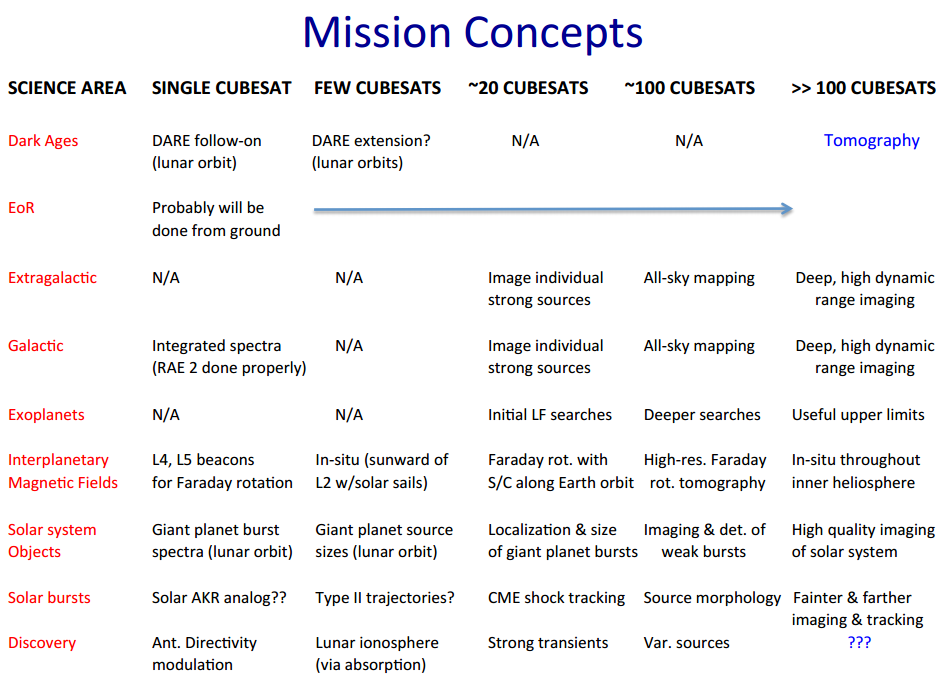
\includegraphics[scale=0.7]{mission_concepts.png}
\caption{Mission concepts for multiple agent systems in all fields (source: \href{http://kiss.caltech.edu/workshops/smallsat2012/presentations/low_freq_missions.pdf}{Presentation by Dayton Jones})}
\end{figure}

\begin{figure}[!ht]
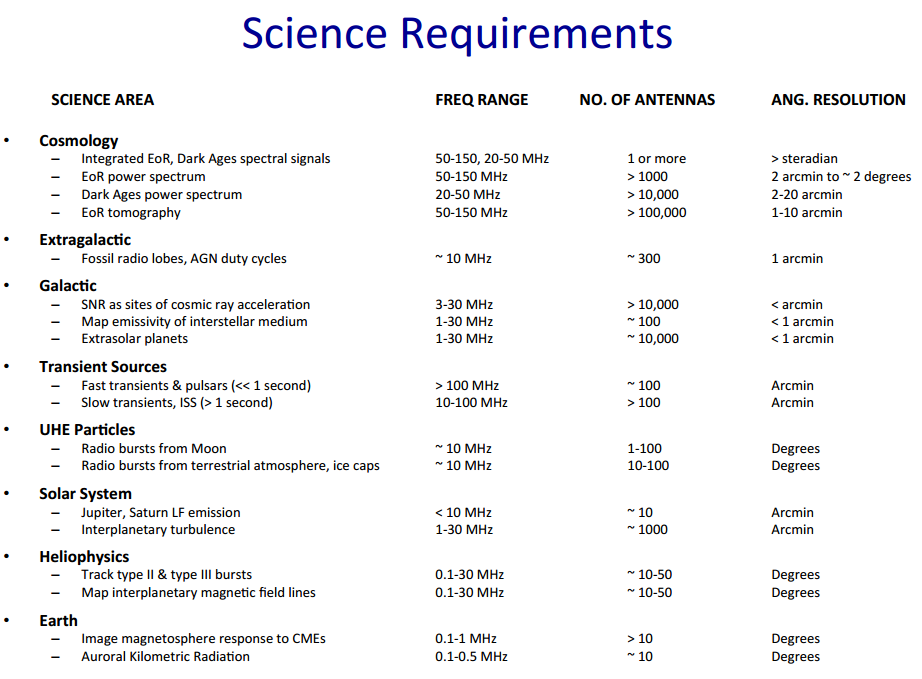
\includegraphics[scale=0.7]{science_req.png}
\caption{Science Requirements for above missions(source: \href{http://kiss.caltech.edu/cosponsored/cubesat2012/presentations/low_freq_science_req.pdf}{Presentation by Dayton Jones})}
\end{figure}
\newpage

\vspace{1cm}
All the missions that have been mentioned above have been plotted on graph as shown below. The vertical axis has the number of satellites that are required to perform that particular mission. The horizontal axis has been split according to whether it can be performed using a single spacecraft or whether formation flying or constellations are required to do the same. They have been colour coded according to the mission class and bigger the size, the costlier the mission. 

\begin{figure}[!ht]
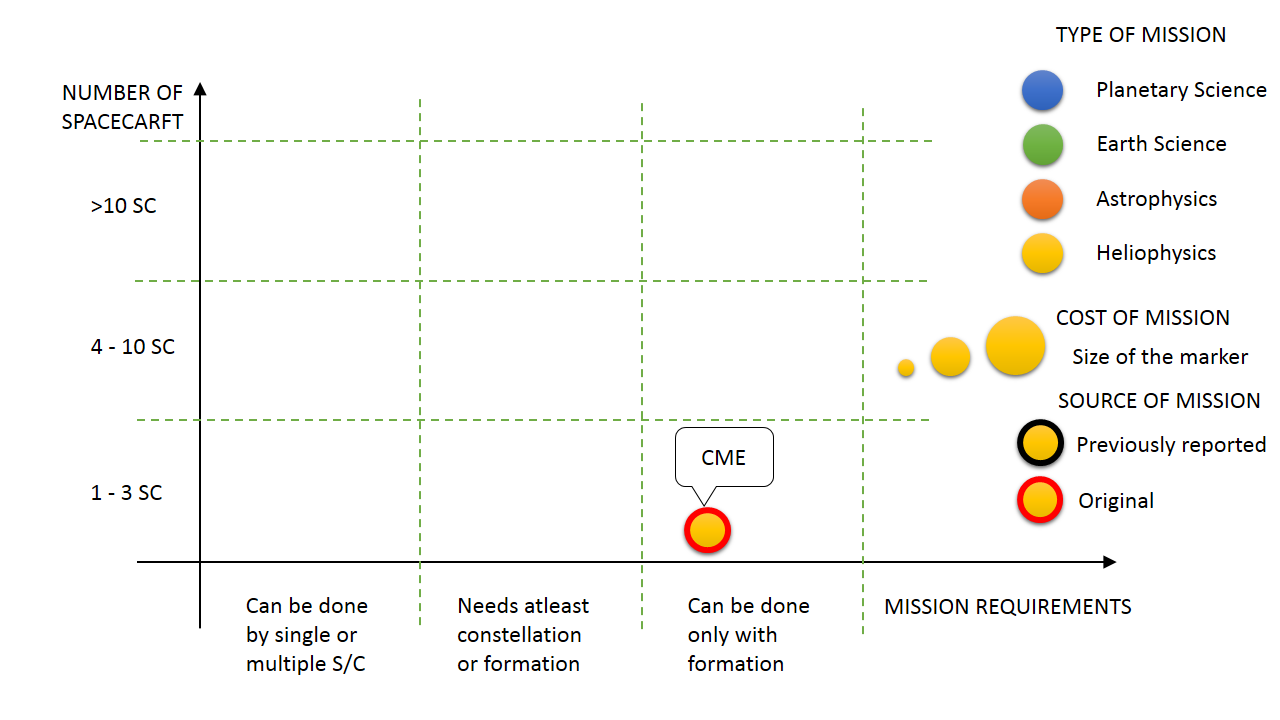
\includegraphics[scale=0.5]{cost_function.png}
\caption{Mission Categorization}
\end{figure}
\newpage
%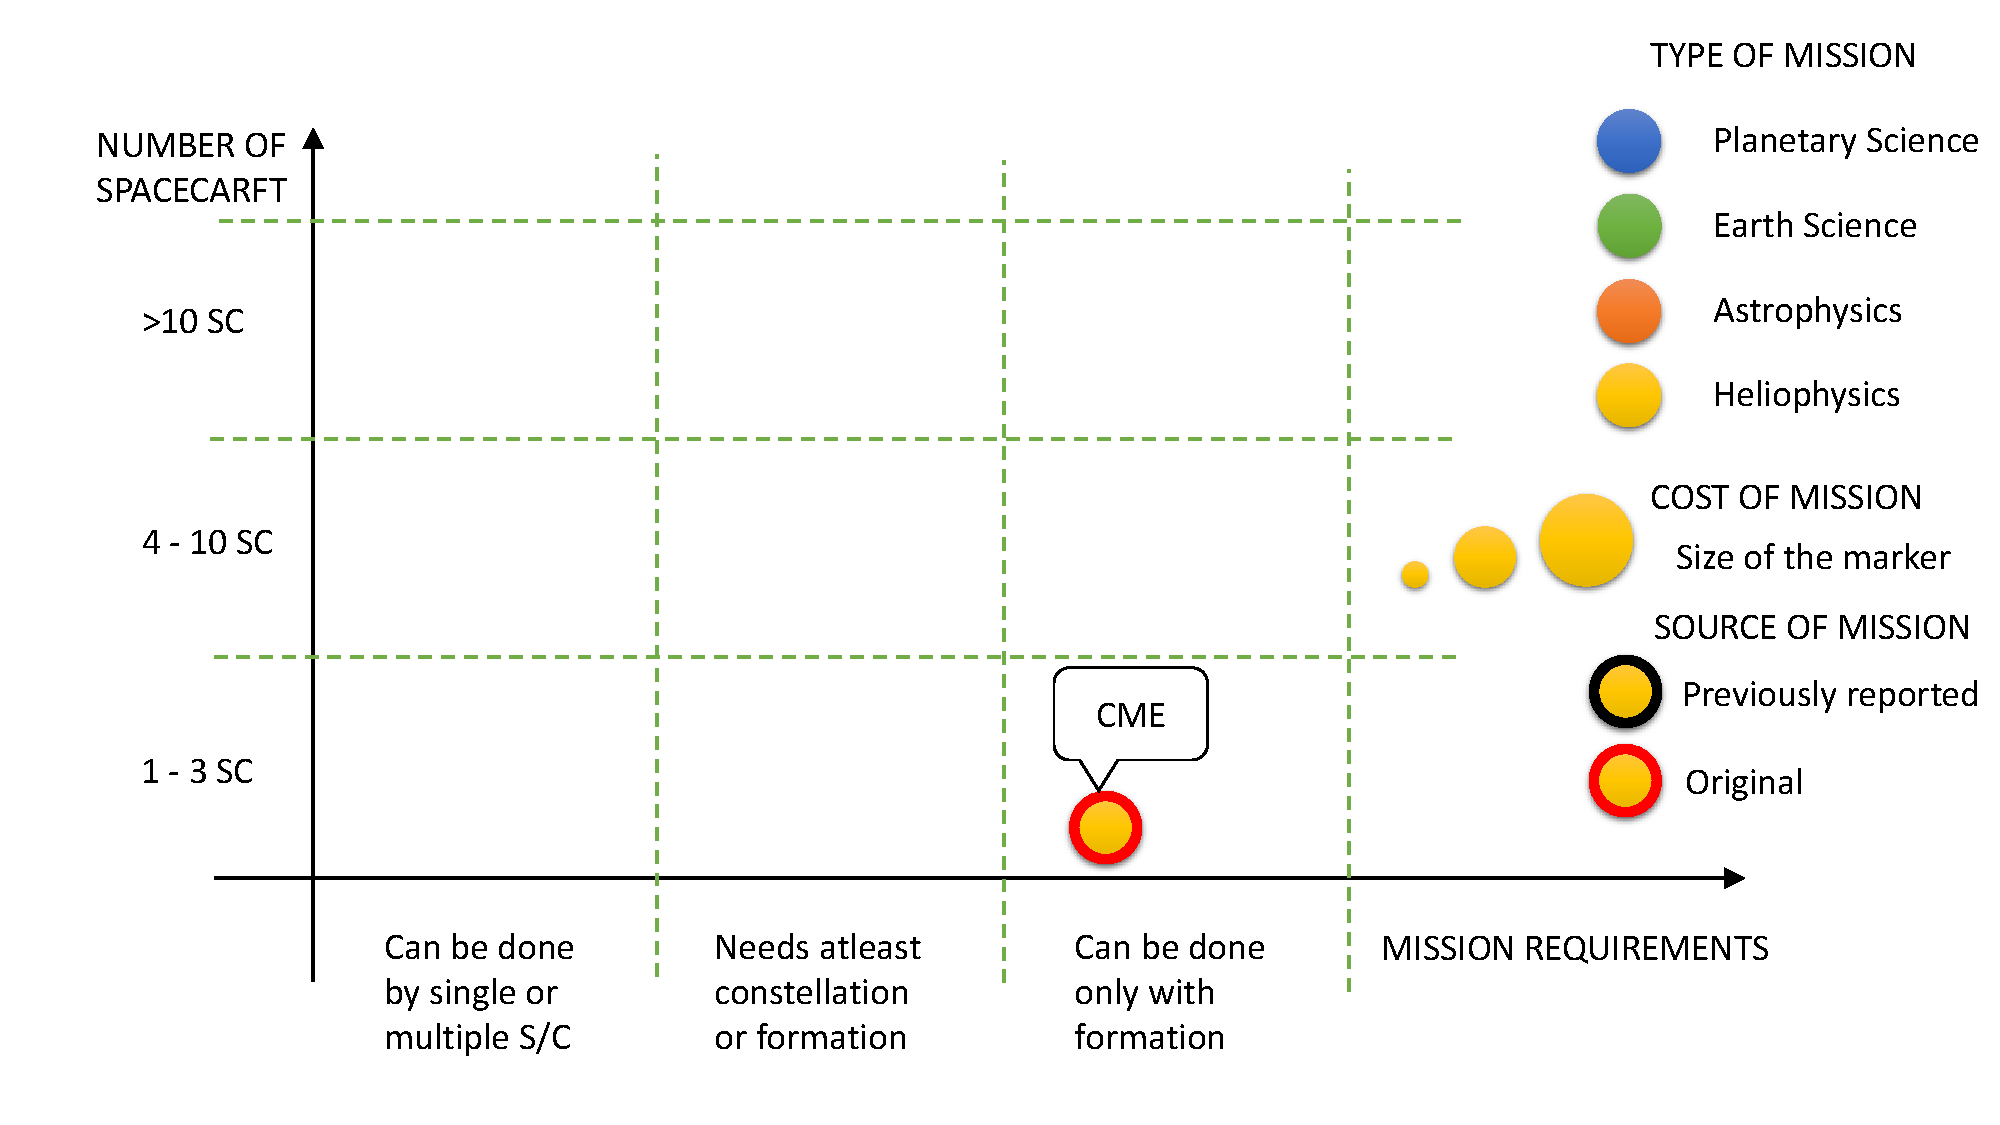
\includepdf[scale = 0.5]{cost_function.pdf}
\section{Our Mission Proposals}

\subsection{Division of Labor in Satellite}
\label{labour}
Every year we throw away satellites because they become worn out. But usually it's only one of the component that causes the problem. The other components work fine but is needlessly thrown away. This makes satellites as one of the major contributors to the build up of space debris. DARPA's Pheonix satellite re-servicing mission addresses these issues and tries to utilize functioning part of the satellites. But instead of trying clean up what has already happened (like  re-using parts of defunct satellites), we propose a mission to reduce problems in the future. The idea is to apply division of labor. Instead of a one big satellite containing all the components, smaller satellites carrying one or two parts could fly in a constellation to represent a system as a whole. Some benefits are listed below: \\

{\bf Expandable:} If more computing power is needed, a CubeSat carrying another CPU could join the constellation. \\
 
{\bf Customizable:} Camera carrying CubeSat could be replaced with a CubeSat with different type of sensor.
If there is free space in terms of data transfer or processing power, same or different company could send in just the sensor unit to collect data. \\

{\bf Reconfigurable:} Working parts could be re-used for different missions.\\

{\bf Green:} Creates less space waste.

\subsection{Satellite Advertising}
\label{ad}
If CubeSats could carry reflective surface or an LED to make itself visible from earth, tightly controlled formation flying CubeSats could spell out a word or even form a display screen in great numbers. Indeed, it would be most likely only visible with the help of a telescope but just the existence of space ad would have great impact on the media. Along with star viewing, it would become "the thing" to look at. Depending on visible areas at that time, different advertisements could be displayed.

\subsection{Orbiting Marker in Space}
\label{marker}
Controlled formation flying satellites could serve as a marker for vision based navigations. Multiple orbiting markers on some other planet could allow better pose estimation than existing star trackers.

\subsection{Graveyard Orbit Transfer Service Formation Flying Proposal}
\label{grave}
\subsubsection{Summary}
At the end of a satellite's service life, a satellite standard exists for the disposal of a spacecraft. For a geosynchronous spacecraft, it is typical to deposit the satellite in an orbit with a perigee altitude above 36,100 km \cite{standard}. This orbit is chosen due to the small $\Delta V$ required to move a spacecraft into the orbit (approximately 7.4 meters per second) and the tendency for the spacecraft to not return to an orbit used by operating spacecraft \cite {SMAD}. Recently however, only about one-third of GEO satellite that have reached the end of their life time have successfully achieved a so called ``graveyard orbit'' \cite{ESA}. The proposed formation flying spacecraft system seeks to increase the percent of spacecraft that successfully maneuver to a ``graveyard orbit'' in a cost effective manner. 

\subsubsection{Concept of Operations}
As a proposed disposal method, consider a satellite in geosynchronous orbit that has just reached the end of its operational life time and cannot move to a graveyard orbit. A formation of CubeSat satellites (used for their extreme cost effectiveness) form together, dock with the dead spacecraft, and fire thrusters to move the dead spacecraft to a graveyard orbit. Because it is difficult to know ahead of time which spacecraft will successfully move themselves to a graveyard orbit and which will not, formation flight is essential to create re-configurable solutions for the many spacecraft that may or may not fail. There will be multiple types of 1U, 2U, and 3U CubeSats. Some CubeSats will serve as attitude and position controllers for the formation once formed together. Others will serve as major thrusters to move the dead satellite out of the geosynchronous orbit. Finally, the remaining CubeSats will act as fuel tanks for the system.

\subsubsection{Proof of Concept CubeSat Mission}
As a proof of concept, a 6U CubeSat could be launched along with three 1U CubeSats. The 6U CubeSat will act as a dead satellite. One of the 1U satellites will serve as a thruster, another as a fuel tank, and the final one as a controller of the formation. The controller will work to form a solution out of the three 1U CubeSats. The re-configured spacecraft will then dock with the 6U spacecraft and move it to a different orbit.


\subsection{Optical Communication Mission}
\label{op_comm}
\subsubsection{Summary}
In the late 1970s, work began on an optical communications technology that could provide orders of magnitude more data transferred from deep space missions than was possible with conventional radio frequency techniques \cite{Hemmati}. Major challenges for such a deep space system include the acquisition, tracking, and pointing for sub-micro-radian accuracy, the use of efficient lasers with moderate power and high modulation rates, and the use of fine-pointing mirrors \cite{FlightRD}. The atmosphere of Earth, additionally, acts as a major obstacle for an optical communications system. Even on a clear day, the atmosphere can significantly attenuate an optical signal. Thus, an optical deep space network will require many more ground stations than the current deep space network. A recent study by Northrop Grumman concluded that even if six ground sites (double the size of the current deep space network) were selected, the array would only be operable 83\% of the time \cite{Wojcik}. Leveraging a formation satellite system in a deep space optical communications network can realistically solve several open problems in optical communication literature and could alleviate major pointing constraints that would be placed on future spacecraft missions if the optical deep space network were constructed.

A formation flying CubeSat mission offers a unique opportunity to demonstrate the technical viability of such a system. Such a mission, if pursued, would allow NASA to make significant progress towards goals laid out by the 2013 to 2022 Planetary Science Decadal Survey \cite{Planetary}. The Jet Propulsion Laboratory is currently conducting a systems engineering study of a base line deep space mission which could demonstrate optical communications technology \cite{Alvarez}. Such a CubeSat mission could add significant value to such a demonstration. Figure 4 displays an overview of the concept of operations of such a deep space formation flight network.
\begin{figure}[!ht]
\centering
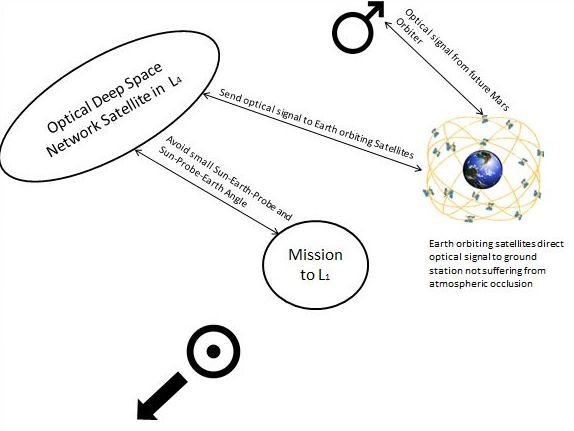
\includegraphics[scale=0.65]{OV1.jpg}
\caption{Mission Concept of Operations Overview}
\end{figure}

\subsubsection{Motivation}
NASA, and in particular the Jet Propulsion Laboratory, has invested significantly in the use of optical communication technology in spacecraft. The scientific community has realized the potential of such a technology and in the 2013 to 2022 Planetary Science Decadal Survey claimed the technology ``would be of major benefit for planetary exploration''. The report also recommends demonstrating such a technology in flight over the next decade \cite{Planetary}. Due to its higher frequencies, optical communication technology is expected to enable the realistic use of synthetic aperture radar as well as other currently unusable remote sensing techniques in Mars and Saturn missions. The technology has an additional benefit of requiring smaller equipment of lower mass \cite{Hemmati2}.

Major challenges with optical communication technology persists, however. Whereas the beam width of a radio signal from deep space may have a diameter on the order of a hundred times the Earth's diameter, optical signals would have a beam width approximately one-tenth the Earth's diameter \cite{Hemmati2}. Additionally, small Sun-Earth-Probe (SEP) and Sun-Probe-Earth (SPE) angles as illustrated in Figure 5 can significantly saturate a signal \cite{Biswas}. Finally, weather on Earth can easily occlude an optical signal and a significant amount of research has been conducted to understand how weather attenuates a signal and how to properly predict the phenomenon \cite{Wojcik} \cite{Shaik} \cite{Hemmati3} \cite{Cowles} \cite{Cowles2} \cite{Cowles3} \cite{Shaik2}. A formation of spacecraft in Earth orbit and located at Lagrange points four and five can mitigate in the impact of the pointing, acquisition, and tracking problem on deep space satellites and can completely solve problems related to inclement Earth weather and small SEP and SPE angles.

\begin{figure}[!ht]
\centering
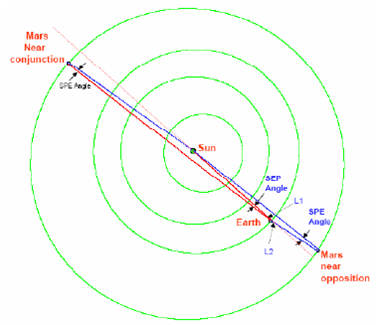
\includegraphics[scale=0.75]{SEPSPE.png}
\caption{Sun-Earth-Probe and Sun-Probe-Earth Angles}
\end{figure}

\subsubsection{Mission Concept of Operations}
An initial concept of such a formation flight system include approximately 24 satellites in Earth orbit. This formation will serve two purposes. First, it will loosen the pointing requirements of a deep space satellite. This is the case, because, instead of using a signal with a beam width on the order of a tenth the diameter of the Earth to point to a small number of ground stations as weather permits, the signal beam can instead transmit to one of the formation satellites. Second, the formation can redirect a signal to a ground station anywhere on the planet. Thus, the impact of weather on the optical deep space network is significantly alleviated. 

The second component of the formation flight system, is a set of satellites located in Lagrange points four and five. These spacecraft will allow deep space satellites experiencing small SEP and SPE angles to redirect their signal to these satellites, which, in turn, redirects the signal to the Earth orbiting formation. Thus, the SEP and SPE angle no longer will limit the operability of such a system.

\subsubsection{Possible Proof of Concept CubeSat Missions}
There are several possible CubeSat missions which could act as a proof of concept mission for the proposed formation flight system. A formation of five 3U CubeSats could be placed in medium Earth orbit. These CubeSats could be equipped with optical communication equipment developed by JPL's Optical Communication Group. One of the CubeSats could be designated as a ``receiver." This receiver CubeSat would transmit optical signals to the ground or to other CubeSats. A distributed decision algorithm could then be used to direct the signal among the CubeSats to one of several ground stations.

An alternative mission could possibly involve collaborating with current work conducted by JPL on the development of a technology demonstration deep space mission. As part of the deep space mission, the JPL satellite would attempt to transmit optical signals to a formation of 3U CubeSats, which would then transmit optical signals to the ground using a distributed decision algorithm which would direct the signal among the CubeSats. 

A final possible mission would be to send one CubeSat to Lagrange point one, a second to Lagrange point four or five, and place a formation of five 3U CubeSats in Earth orbit. Such a mission would demonstrate how a formation flying deep space optical network would solve the small SEP and SPE angle problem discussed in previous literature.




\subsection{Fixed Satellite Service in Maintenance and Repair Industry}
\label{mro}
\subsubsection{Summary}
The commercial satellite industry is a large and relatively stable sector of the space industry providing services such as satellite television, radio, and broadband. These three applications alone are a \$93.3 billion industry \cite{SIA}. These satellites, meanwhile, are extremely costly for any corporation. A geosynchronous satellite such as the DirecTV-5, could very well cost in the neighborhood of \$300 million \cite{SMAD}. The product line proposed in this paper, reduces the risk involved with such a system by offering a service to satellite service companies to purchase an attitude control insurance package. Thus, in the event of a failure in a satellite's attitude control system, the service would fix that satellite's system to ensure continued operation. 
 
\subsubsection{Motivation}
To motivate the need for such a service for satellite operators, consider the satellite TV service company DirecTV. This company operates a fleet of satellites on missions greater than ten years. As of 2012, the company has insurance to cover the unamortized  book value of a satellite in the event of a premature loss. However, the insurance does not cover the loss of revenue due to the loss of a satellite. Assuming a ten year mission, with a \$300 million total mission cost and 17\% profit margin. The loss of a satellite would on average cost the company \$5.1 million in revenues every year \cite{DirecTV}. Thus, the current proposal acts as an improvement on current insurance practices by not only insuring against the unamortized book value of a satellite, but also preventing the lost revenue the company would experience. 

\subsubsection{Concept of Operations}
The improved satellite service solution would require a formation flight of many spacecraft. There would exist two kinds of spacecraft: a 1U satellite whose volume is dominated by a reaction wheel, torque rod, or control moment gyroscope (it will be assumed a reaction wheel is the chosen method of actuation) and a 2U satellite controller. The cubesat standard is used to capitalize on cost advantages. The 1U satellite will be passively stabilized to eliminate the need for any use of volume beyond a reaction wheel. The 2U satellite will contain all computing, thrusting, and other capabilities of a standard spacecraft. When a  customer's satellite fails, the insurer would compute an optimal configuration by which attitude control could be regained. The passively controlled or position controlled formation would then reform into an attitude control solution and it would dock with the damaged spacecraft, which would then be repaired.

Technical challenges of such a project include optimal control of the formation, the customization of a solution for a broken spacecraft, and how the 2U satellite forms a solution for the broken spacecraft. Docking with the broken spacecraft and the subsequent control of the customer's spacecraft can also be a challenge.

To prove the cost model of this concept, consider DirecTV again. A \$300 million satellite on a ten year mission has an 18\% probability of experiencing failure due to the attitude control system. While failure is not equally likely throughout the ten years, failure before the end of year five is 11\% \cite{SMAD}. Thus, such a service would be worth upwards of \$27 million per satellite. Assuming a cost of \$150,000 per 1U satellite, a cost of \$300,000 per 2U satellite (each with a mass of 1 kg), and a launch cost of \$3,409 per kilogram (on a Dnepr-1 rocket), launching a 100 kg formation would cost under \$16 million. Assuming 25\% of the formation is used by one satellite on average and the service charges \$16 million for a 10 year policy, the company would make an average \$1.2 million dollars a year per satellite. Now consider if the insurer contracted with DirecTV (12 satellites), EchoStar (22 satellites), SES S.A. (53 satellites), and INTELSAT (59 satellites). Such contracts would require 3650 satellites to be produced and an average yearly profit of \$175.2 million could be anticipated. 

\subsubsection{Proof of Concept CubeSat Mission}
For an initial proof of concept, a mission involving 5 CubSats is proposed. The first CubeSat is a 3U satellite such as ExoplanetSat shown in Figure 6. This 3U CubeSat will experience an attitude control failure during the mission. A 2U satellite will then create a solution from three 1U CubeSats. This solution will dock with the 3U CubeSat and provide attitude control. Additionally, inflatable structures could be placed on the 3U CubeSat so that its size is closer to a potential customer satellite.

\begin{figure}[!h]
\centering
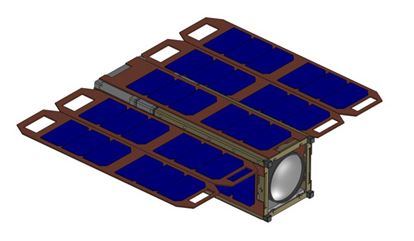
\includegraphics[scale=0.75]{ExoPlanetSat.jpg}
\caption{ExoPlanetSat \cite{MIT}}
\end{figure}


\subsection{3D Printing Replacement Parts For Dying Satellites}
\label{3d}

When satellites start to degrade or suffer from micrometeoriod impacts, replacement parts can revitalize a satellite that would otherwise need to be deorbited. Launching replacement parts can be expensive, in some cases more expensive than launching a new satellite. 3D printing new pieces for eligible satellites would reduce the upkeep costs of satellite constellations and potentially reduce the orbital debris.  

3D printing technology for space (by Made In Space) is slated to be tested in orbit in 2014 and has already succeeded in parabolic flight tests. Limitations may exist as to size and placement of replacement part on the satellite, so it may be necessary to study a set of satellites with common buses, like TDRSS or GPS to assess what parts are possible to replace. 

The satellite formation would have one or more satellites dedicated to printing and other satellites dedicated to removing and replacing the part on the broken satellite. The 3D printing could occur while the satellites travel to the orbit of the broken satellite. Formation flying would be necessary during the hand-off of the part and possibly also during the printing itself depending on the requirements of the printer. 

\subsection{Tracking Gamma Ray Bursts (GRBs)}
\label{grb}
A formation could be used to source GRBs through precise triangulation. With accurate measurements of inter-satellite distance and GRB incident time, the satellites could potentially increase the accuracy of GRB detection and positioning. \cite{Ref:Dill}. This mission has since been proven unnecessary, because current satellites use gamma ray detectors and UV detectors together, with the UV detectors calculating the positioning. A formation of gamma ray detectors can still be useful to verify the measurements of current satellites like NASA's Fermi, or possibly to address gaps in coverage. 

The gamma ray detector formation could also look for gamma rays emitted by thunderstorms. Fermi has observed the phenomenon, but it could possibly do with more study, to help Fermi differentiate between the real gamma ray signals and the thunderstorm generated gamma rays.\cite{Ref:Fermi} \cite{Ref:Kitts}

\subsection{Tomography of the Ionosphere/Auroras}
\label{tomography}

Depletion in ionospheric plasma can disrupt signal transferrance,
and not much is known about the depletion zones. The formation would
study how the depletions change and propagate so that scientists can
create a model and further their understanding of the phenomenon.
The satellites would be in a 360 km orbit at an inclination of 52
degrees \cite{Ref:Krause}\cite{Ref:Bracikowski}. These measurements
can also help to show the interactions between the thermosphere and
ionosphere \cite{Ref:Blalthazor}. 

Currently scientists studying auroras have to collapse their 3D models
into two dimensions to verify them. The tomography created by the
formation would allow the scientists to verify their models in 3 dimensions,
much more accurately than the current process. 


\subsection{Inflatable De-Orbit Device}
\label{inflatable}

A formation of satellites could be used to test an inflatable, such
as a de-orbiting device. Some of the satellites would not have inflatables
to determine the difference between the satellites with de-orbiter
and those without. The formation would not only test the inflatable
deployment, but also the efficacy against standard orbit degradation. 

\subsection{Variable-Range Solar Coronography}
\label{coronograph}
Coronal mass ejections (CMEs) are a common phenomena in our Sun and
they can have a significant impact in our daily life. CMEs release
enormous amounts of plasma and energy into space inducing violent
solar winds. If this wind reaches our planet it can alter the Earth's
magnetosphere, cause remarkable aurora and malfunctioning in electrical
distribution lines, interfere in our communications and even damage
our satellites. For these reasons, the ability to predict and model
the influence of CMEs on the Earth is of great importance. Therefore,
several space missions are currently dealing with this issue, such
as:
\begin{enumerate}
\item Solar and Heliospheric Observatory (\href{http://www.nasa.gov/mission_pages/soho/index.html\#.UjUrV8YagWA}{SOHO}):
it is a monolithic spacecraft located at the first Lagrangian point
(L1) and constantly facing the Sun. Among the various instruments
that SOHO carries there are several that are dedicated exclusively
to study the solar corona:

\begin{enumerate}
\item Large Angle and Spectrometric Coronagraph (\href{http://lasco-www.nrl.navy.mil/}{LASCO})
has become one of the most relevant instruments in SOHO. It consists
of three different coronographs that focus their attention on a different
area around the solar corona. Finally, the data and images collected
from these three coronographs in three different nested regions around
the Sun is blended to create a single image and data collection. In
the following table there are several characteristics of these coronographs:


\begin{table}[H]
\begin{centering}
\begin{tabular}{|c|c|c|c|c|c|}
\hline 
\multirow{2}{*}{\textbf{Coronagraph}} & \textbf{Field of View} & \textbf{Occulter} & \textbf{Spectral} & \textbf{Objective} & \textbf{Pixel }\tabularnewline
 & \textbf{($R_{sun})$} &  & \textbf{ Bands} & - & \textbf{Size}\tabularnewline
\hline 
\hline 
C1 & 1.1-3.0 & Internal & Fabry-Perot & Mirror & 5.6''\tabularnewline
\hline 
C2 & 1.5-6.0 & External & BroadBand & Lens & 11.4''\tabularnewline
\hline 
C3 & 3.7-30 & External & BroadBand & Lens & 56.0''\tabularnewline
\hline 
\end{tabular}
\par\end{centering}

\caption{LASCO Coronographs \cite{LASCO_Coronal_Imaging_Spectroscopy}}


\end{table}


\item Coronal Diagnostic Spectrometer (\href{http://solar.bnsc.rl.ac.uk/}{CDS})
performs spectrometry of the atoms and ions in the solar corona and
the transition region.
\item Ultra Violet Coronagraph Spectrometer (\href{http://www.cfa.harvard.edu/uvcs/}{UVCS})
measures the spectrum characteristics of the highly ionized plasma
in the solar corona, studying a region between 1.3 and 12 solar radii.
\end{enumerate}
\item Solar Terrestrial Relations Observatory (\href{http://www.nasa.gov/mission_pages/stereo/main/index.html\#.UjUnXsYagWA}{STEREO})
consists of two spacecraft that simultaneously take pictures of the
solar corona from different positions in their orbit. Having two spacecraft
looking at the same region has allowed this mission to create the
first stereoscopic views of CMEs and other solar measurements. 
\end{enumerate}
The coronagraphs implemented in these missions have two main limitations.
The first is that for a fixed distance between the occulter and the
imaging sensor, the instrument is only capable of providing images of
a finite region above the Sun's limb. Furthermore, if the instrument
is focused on the study of the closest layers above the Sun's limb,
the majority of the imaging element is shadowed by the occulting disk.
The second limitation is the aperture due to size restrictions. Consequently,
LASCO instrument includes three different coronographs with nested
fields of view to create a full picture of the desired region around
the Sun. Furthermore, LASCO is not able to provide stereoscopic images
of CMEs, whereas STEREO does provide stereoscopic images, as it consists
of two different spacecrafts, but only focuses on a certain region
of the Sun's corona.

\textcolor{black}{Formation flying satellites could mean a great leap
in the study of the solar corona and CMEs. A range-variable stereoscopic
coronagraph could be implemented with 4 formation flying satellites.
Separating the occulter disk and the imaging element in two different
spacecrafts will allow heliophysicists to focus their instrument on
the desired area and even follow CMEs as they expand into space just
by varying the distance between the spacecraft containing the occulter
and the imaging element. Moreover, adding a pair of occulter and imaging
spacecraft the mission will be able to provide stereoscopic images
of CMEs. As we keep adding more spacecraft to the formation, the mission
can either improve the stereoscopic data or enhance the field of view.}

\scalefig{Formation_Flying_Coronagraphs.jpg}{0.5}{Range-variable stereoscopic coronagraph}
\newpage

\textcolor{black}{To estimate the attitude requirements of this kind
of mission, the following restrictions have been imposed. The occulter
has to maintain a position in which the imaging sensor is never exposed
to Sun's direct radiation. Therefore, the occulter shadows a circle
equivalent to$1.05R_{sun}\text{\textpm}0.025R_{sun}$. To do so, we
propose a simplified system of 2 formation flying satellites with
3 DOF ($d,\theta,\delta)$ represented in Figure 8}


\scalefig{FF_Coronograph_DOF.jpg}{1}{DOF for two Formation Flying Satellite Coronagraph}

\textcolor{black}{The following table contains an estimation of the attitude requirements for a formation of two CubeSats, assuming $\theta=1\text{º}$:}

\begin{table}[H]
\centering{}%
\begin{tabular}{|c|c|c|c|c|c|c|c|c|c|c|}
\hline 
\multicolumn{2}{|c|}{Radius of occulter (m)} & \multicolumn{3}{c|}{0.243} & \multicolumn{3}{c|}{0.487} & \multicolumn{3}{c|}{0.974}\tabularnewline
\hline 
\multicolumn{2}{|c|}{$d_{max}$(m)} & \multicolumn{3}{c|}{50} & \multicolumn{3}{c|}{100} & \multicolumn{3}{c|}{200}\tabularnewline
\hline 
\multicolumn{2}{|c|}{$\text{\ensuremath{\Delta}d}$(\%)} & $\text{\textpm}1$ & $\text{\textpm}0.1$ & $\text{\textpm}0.01$ & $\text{\textpm}1$ & $\text{\textpm}0.1$ & $\text{\textpm}0.01$ & $\text{\textpm}1$ & $\text{\textpm}0.1$ & $\text{\textpm}0.01$\tabularnewline
\hline 
\hline 
$\delta$(m) & $\Delta\delta$(\%) & \multicolumn{9}{c|}{$\Delta\theta$(º)}\tabularnewline
\hline 
\multirow{3}{*}{0.1} & $\text{\textpm}1$ & - & - & - & - & 0.0022 & 0.0032 & 0.0133 & 0.0135 & 0.0135\tabularnewline
\cline{2-11} 
 & $\text{\textpm}0.1$ & - & 0.0166 & 0.0194 & 0.0112 & 0.0207 & 0.0216 & 0.0225 & 0.0228 & 0.0228\tabularnewline
\cline{2-11} 
 & $\text{\textpm}0.01$ & - & 0.203 & 0.0231 & 0.0131 & 0.0225 & 0.0235 & 0.0234 & 0.0237 & 0.0237\tabularnewline
\hline 
\multirow{3}{*}{0.01} & $\text{\textpm}1$ & 0.0138 & 0.0191 & 0.0196 & 0.0138 & 0.0210 & 0.0217 & 0.0138 & 0.0219 & 0.0227\tabularnewline
\cline{2-11} 
 & $\text{\textpm}0.1$ & 0.0175 & 0.0228 & 0.0233 & 0.0157 & 0.0228 & 0.0235 & 0.0147 & 0.0228 & 0.0236\tabularnewline
\cline{2-11} 
 & $\text{\textpm}0.01$ & 0.0179 & 0.0232 & 0.0237 & 0.0158 & 0.0230 & 0.0237 & 0.0148 & 0.0229 & 0.0237\tabularnewline
\hline 
\multirow{3}{*}{0.001} & $\text{\textpm}1$ & 0.0138 & 0.0228 & 0.0237 & 0.0138 & 0.0228 & 0.0237 & 0.0138 & 0.0228 & 0.0237\tabularnewline
\cline{2-11} 
 & $\text{\textpm}0.1$ & 0.0138 & 0.0228 & 0.0237 & 0.0138 & 0.0228 & 0.0237 & 0.0138 & 0.0228 & 0.0237\tabularnewline
\cline{2-11} 
 & $\text{\textpm}0.01$ & 0.0139 & 0.0228 & 0.0237 & 0.0138 & 0.0228 & 0.0237 & 0.0138 & 0.0228 & 0.0237\tabularnewline
\hline 
\end{tabular}\caption{Estimated requirements for two Formation Flight Satellite Coronagraph}
\end{table}


In summary, the mission requirements obtained are achievable with current
sensors and actuators available on the market. The proposed mission
is feasible and could lead to a great improvement in the flexibility
and data collection of heliophysics missions.


\subsection{CubeSat landing swarm to track and model asteroid belts}
\label{ast_belt}
An example of the current interest in the asteroid belt among the
scientific community is the NASA's \href{http://dawn.jpl.nasa.gov/mission/journal.asp}{Dawn} mission.
This mission has already placed a spacecraft orbiting around the gigantic
asteroid Vesta and now heading towards Ceres, where it is expected
to unveil some of the interesting aspects of this body. Ceres is thought to be
an icy dwarf planet capable of providing a reasonable explanation about
the origin of water in Mars and Earth. Therefore, Ceres and some of
the asteroids in this belt are quite interesting from an astrobiological
point of view as they contain ice water. In addition, some asteroids
have considerable amounts of metals and carbon compounds. Scientists believe
that this region holds some important clues about the origin and evolution
of the Solar System. Nevertheless the only outstanding mission to
the asteroid belt indicates that there is still much work to be done to answer
all the questions scientist ask now. For that reason, a swarm of CubeSats
is a promising way to continue the exploration of the asteroid belt
in an efficient and flexible way.

A swarm of CubeSats capable of landing on several asteroids has many
profitable applications although initially flight formation will not
be needed, the mission could be notably improved with the aided help
of cooperating spacecrafts:
\begin{enumerate}
\item In an initial approach the CubeSats could provide accurate imaging
and mapping of a wide variety of asteroids. After landing on the surface
of the asteroid samples of them could be taken in order to study composition
and origin.
\item The swarm of CubeSats spread all over the asteroid belt could be used
to easily track smaller asteroids, improve the computational models
of the asteroid belt and precisely estimate collisions or orbital
variations of different asteroids.
\item These small satellites could be used to improve communications with
more distant spacecraft and even create a network all around the asteroid
belt. This will allow easy communications with spacecraft even though
the Sun is in the way between the Earth and the spacecraft and therefore
blocks the incoming and outgoing signals.
\item There has been much speculation about the industrialization of the
asteroid belt and how this could supply materials and energy to missions
in Mars or beyond. The swarm of CubeSats could set the foundation
of this movement. Stackable CubeSats can lead to machine construction
and consequently to the asteroid belt industrialization.
\end{enumerate}

\subsection{Sun Energy Collector}
\label{energy_collector}
Harvesting energy has been and is still one of the critical aspects
of a space mission. Some examples of this problem are: 
\begin{enumerate}
\item The Mars Rover Opportunity, unable to perform its experiments on the
slopes of mountains and sand dunes where the sun does not shine during
the day. Hence, the mars rover has experienced important limitations
in its operations due to energy restrictions.
\item Spacecraft traveling to the outer Solar System or even out of the
Solar System require important amounts of energy for their propulsion
systems in order to gain the needed velocity. Furthermore, the moons Europa and Enceladus, are thought
to hide liquid water beneath their frozen surfaces and, therefore, have
been classified as high priority for NASA and ESA. Consequently, there
is an obvious need for cheaper sources of energy for interplanetary
missions.
\item Satellites charge their batteries while exposed to the Sun's radiation.
Then, when entering the night-side of a planet for a long period
of time, satellites are sometimes forced to perform their science with low-power
modes in order to save energy.
\end{enumerate}
A group of formation flying satellites with deployable mirrors could
be the solution for this scarcity of energy. The Sun is a constant
and powerful source of energy in space. Accordingly, spacecraft and
ground systems could benefit more from the Sun's energy than they
are doing now. An orientable array of mirrors could be implemented
in several spacecraft to provide energy to a wide range of missions:
\begin{enumerate}
\item Satellites in desperate need of energy could be rescued from thousands
of kilometers away just by re-orienting the formation flying spacecraft.
Or even better, critical satellites could be able to perform all their
experiments during long periods in the dark side of a planet. 
\item Vehicles and rovers on other planets or moons will have the ability
to continue their research during the night and after long periods
in shaded areas. For this, placing a group of formation flying satellites
in orbit around the corresponding planet or moon will enable pointing
a beam of light to those vehicles that require energy.
\item A beam of photons could be carefully pointed toward a solar sail to
increase solar pressure and help the classical propulsion systems
take the spacecraft to the outer Solar System. By this means, space
agencies would be able to save millions of dollars in putting large
quantities of combustible into space.
\item A group of formation flying satellites could be used as a test-bed
to determine how light can be used to deviate a small asteroid from
its trajectory.
\end{enumerate}


\subsection{Space Wake studies}
\label{space_wake}
The vacuum that has been generated by the best vacuum generators on ground have gone only
go upto a particular level of purity. However, we can use the naturally available vacuum in
space. The problem is that the vacuum available in LEO is not very pure. High purity vacuum
can be obtained in higher orbits, but it is not feasible to reach those with CubeSats. This idea
is that we can have a CubeSat with an inflatable disk-like structure, orbit around the earth in
LEO. Studies show that this produces very highly pure vacuum in it's wake. We can have the
other CubeSats follow in this wake to conduct any required experiments. Possible applications
are: Understanding atmospheric density distribution, understanding wake patterns of satellites,
producing highly pure materials etc. Formation flying is useful for this mission, it can be
performed in LEO and 4-5 CubeSats might be ideal for it (depending on the application). A
representational image has been shown in Figure 9. 
\scalefig{space_wake.png}{0.9}{Space wake studies concept}

The first or leader CubeSat in the above figure is denoted by 1. The oval denoted by 2 in
the figure is the inflatable structure. The earth is shown below and the direction of motion is
also indicated. CubeSats 3, 4 and 5 will follow in approximately that formation. The white line
extending from the end of the inflatable structure is just a representation of the wake created
(Note: This may not be how the wake actually looks). Each of the CubeSats will have a sensor
in front of it which can measure the drag felt by it (I am not yet sure what this sensor would
be). CubeSat 3 and 4 would feel less drag as they are in the immediate wake of the leader.
CubeSat 5 would feel much more than 3 and 4 as it is farther away. Thus using the differential
drag measurements of the leader and CubeSats 3 and 4, a density model of the atmosphere can
be generated. A study on the how much drag is felt by CubeSat 5 while varying the distance between the leader and CubeSat 5 can also be done. We can also have additional CubeSats along the z axis using which we can measure the 3D variations.

\subsection{Open source CubeSat Testbed}
\label{testbed}
We can have a mission in which we launch a set of 4-5 CubeSats in LEO flying in a basic formation. The architecture of these CubeSats will be open to the public so that anyone can write code for it. The limitations and the capabilities of the CubeSats will be clearly listed and everyone would have to follow it. They can send us the code and we can then upload it to the CubeSats which will perform them in real time. This is like a tested for CubeSat algorithms. A lot of people now would have algorithms that they would like to test, but might not have access to satellites. This is again ideal for us as it's in LEO, 4-5 CubeSats will be sufficient and formation  flying is essential. The second advantage of this is the additional source of funding which can be charged for people to test their code on our testbed. The third advantage is that it will just be a technology demonstration from our end without having to worry much about the physics or science behind the missions, thus allowing us to define the requirements. The problem is that, the lifetime of the testbed would be low as of now ( 1-2 months). However, it is a reasonable assumption that this would increase as new technologies are developed.


%\section{Actuators and Sensors}

Below are attached the images that have been found regarding this. They are taken from the presentations given by \href{http://kiss.caltech.edu/workshops/smallsat2012b/presentations/mueller.pdf}{J.	Mueller} and \href{http://kiss.caltech.edu/workshops/smallsat2012b/presentations/bennett.pdf}{Matt Bennett}. 

\begin{center}
\begin{figure}[!ht]
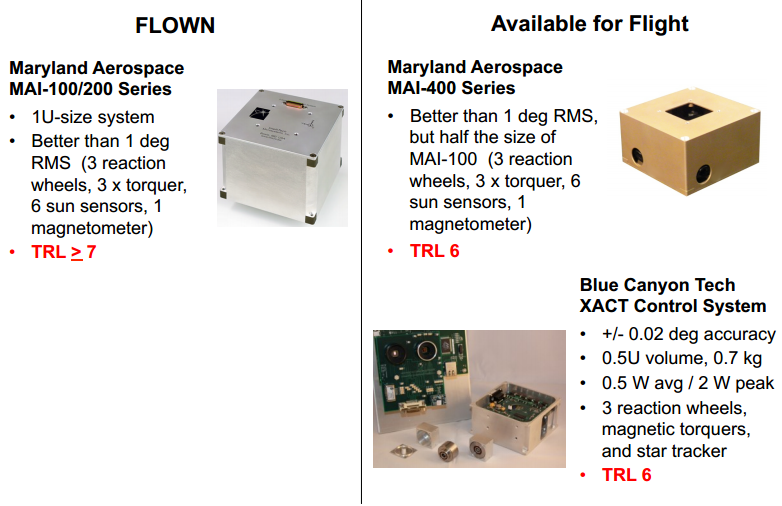
\includegraphics[scale=0.8]{attitude_control.png}
\caption{Current attitude control sensors and actuators}
\end{figure}
\newpage
\begin{figure}[!ht]
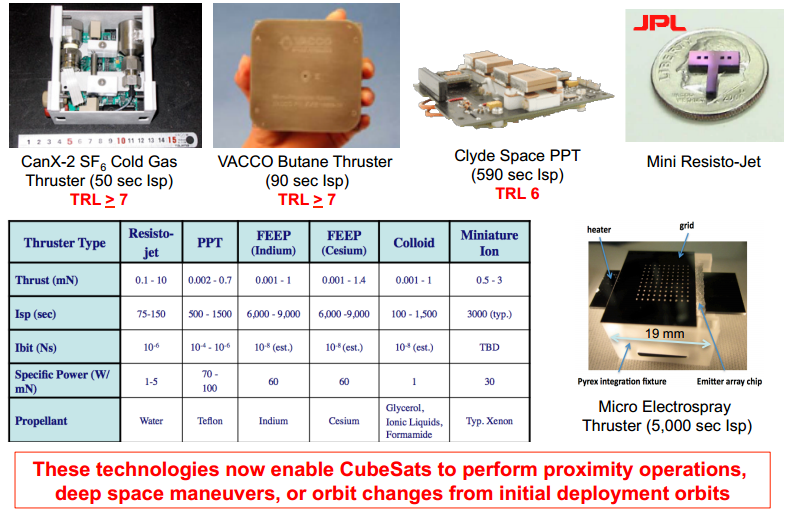
\includegraphics[scale=0.7]{prop_available.png}
\caption{Current thrusters}
\end{figure}
%\newpage
\end{center}
\newpage

\begin{figure}[!ht]
\begin{center}
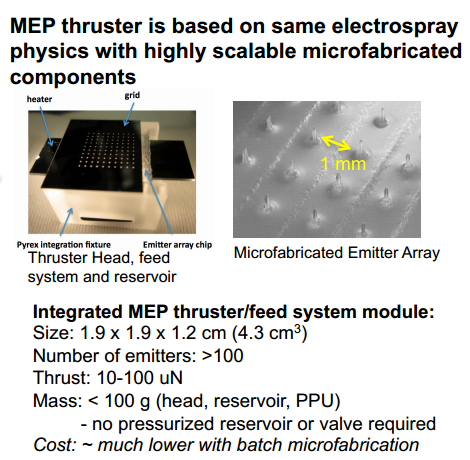
\includegraphics[scale=0.7]{MEP_prop.png}
\caption{Micro-Electric Propulsion specifications}
\end{center}
\end{figure}
\newpage
This is not available of the shelf as of now. They had said it will take 1-2 years in December 2012. It will be a TRL 6 when it becomes available.  

Given below is a table showing what can be achieved using the state of the art controllers and actuators(as on December 2012). 

\begin{figure}[!ht]
\begin{center}
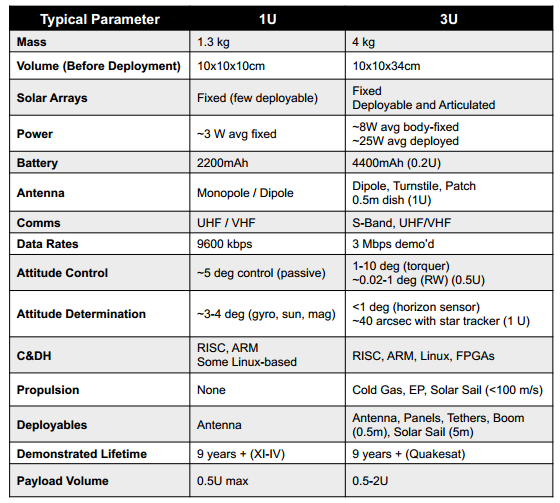
\includegraphics[scale=0.7]{state_of_art.png}
\caption{Current state of the art in all fields}
\end{center}
\end{figure}
\newpage
%%% Comment:
%\documentclass[english]{article}
%\usepackage[T1]{fontenc}
%\usepackage[latin9]{inputenc}
%\usepackage{babel}
%\usepackage{pdfpages}
%\usepackage{float}
%\usepackage{graphicx}
%\usepackage{mathtools}
%\usepackage[margin=0.5in]{geometry}
%\begin{document}
%
%\title{Sensors and Actuators}
%
%
%\author{David Hanley and Hong-Bin Yoon}
%
%\maketitle

\section{Actuators and Sensors}
Listed in this part of the report is a set of sensors, actuators, and thrusters that could potentially be used on Cubesats from 1U to 3U. There is a wide range of sensors and actuators available for use depending on size, weight, and performance constraints. While thrusters currently on the market are generally of a lower technology readiness level than the available sensors on the market, there are still a range of options among available thrusters to choose based on size, weight, and performance constraints as well. 

Additionally, there are several integrated attitude determination and attitude control products available on the market. These systems usually are quite compact and contain star trackers, sun sensors, and reaction wheels among other sensors and actuators. Finally, the end of this report presents a short list of general suppliers that can be considered in the future for sensor and actuator parts as well as parts for other systems on the cubesat. 

\subsection{Inertial Measurement Unit(IMU)}

%% IMU(gyro, accelero, magneto, baro..etc)
Most Inertial Measurement Unit(IMU) or Inertial Navigation System(INS) include sensors for both position estimation and attitude estimation. \\\\

%%Silicon Sensing IMU

\begin{figure}[h!]
   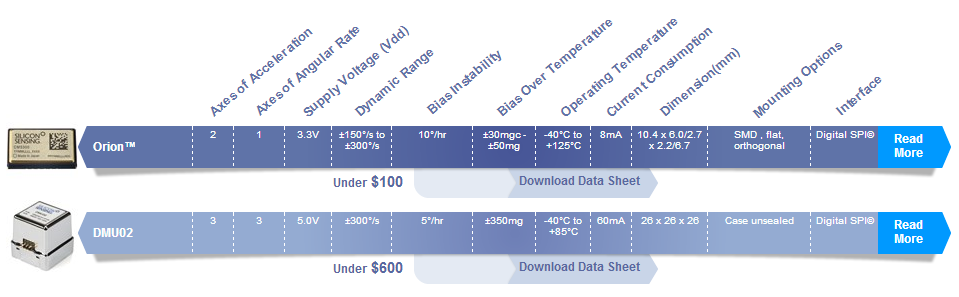
\includegraphics[scale=0.6]{IMU/siliconSensing_IMU.PNG}
   \caption{IMU's from Silicon Sensing \cite{imu1}}
\end{figure}


%% Analog Devices IMU + Gyro + accelo
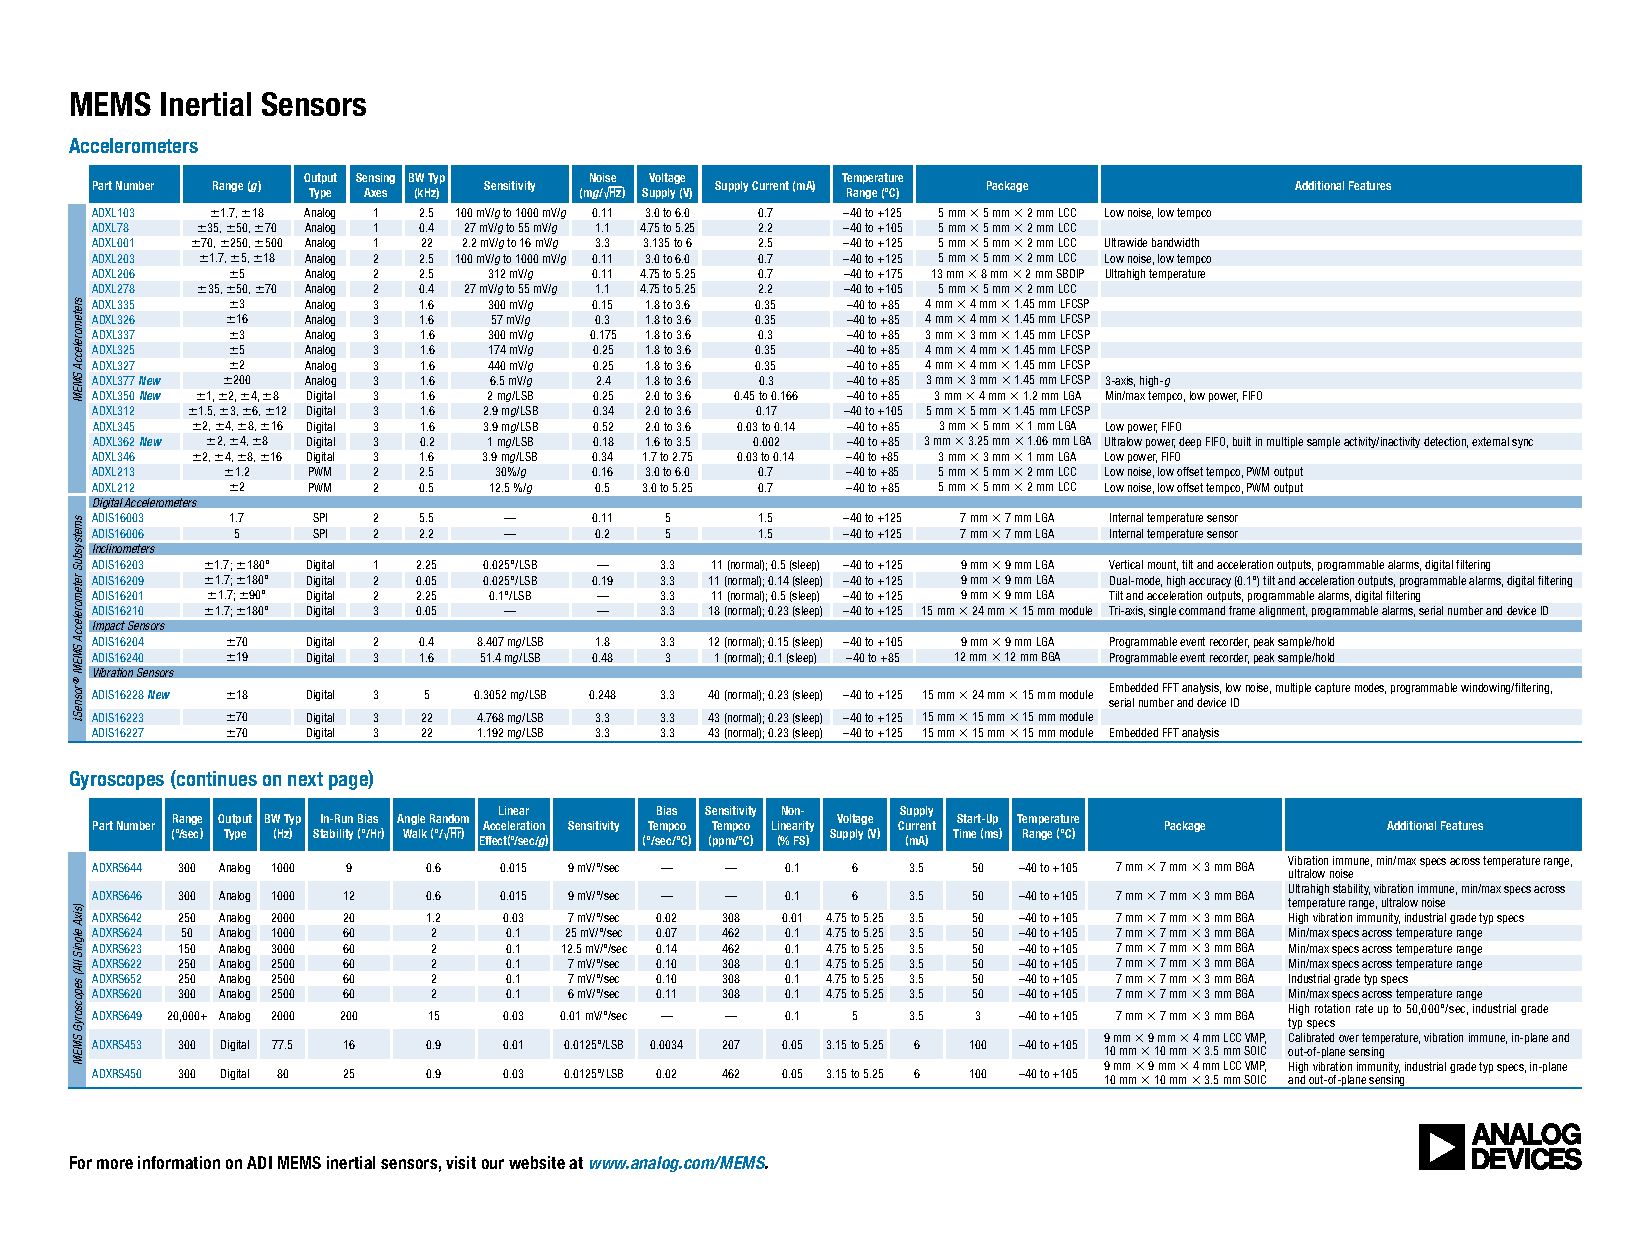
\includepdf[pages={1,2}]{IMU/AnalogDevices_Full_List.pdf}
Information from \cite{imu2}.

\subsection{Position Estimation Sensors}
%% List GPS
\begin{center}

     \begin{tabular}{ |p{2cm} | p{1cm} | p{2cm} | l | l | l | p{5cm} |}
     \hline

      {\bf Name} & {\bf Mass} & {\bf Size} & {\bf Accuracy} & {\bf Type} & {\bf TRL} & {\bf Comment}  \\ \hline

     Aerocube-4 GPS \cite{Gangestad} & NA & NA &  {$ \pm 20 $} & GPS receiver & NA & Orbit determination once per day or as power system permits \\ \hline

     Nano Star Tracker on Chip (STC) \cite{Prokhorov} & 65 g & 73.5x 57.0x 57.8 mm & 10''~50'' & Star Tracker & NA & 19.5 deg field of view, update rate 10 Hz, mean power (without Peltier cooler 250mW), peak power 1 W \\ \hline
     \end{tabular}
     \captionof{table}{Available position estimation sensors}
\end{center}

\subsection{Attitude Estimation Sensors}
%% List Star Trackers and Sun, Earth sensors, magnetometer.
Some attitude estimation sensors and actuators were obtained from the small satellite conference organized by KISS in 2012. They are shown in the image given below.  Apart from this, a table containing actuators and sensors from other sources has also been given below. 
\scalefig{attitude_control.png}{1}{Current attitude control sensors and actuators (source: \href{http://kiss.caltech.edu/workshops/smallsat2012b/presentations/bennett.pdf}{Presentation by Matt Bennett})}

\begin{center}
     \begin{tabular}{ | p{2.25cm} | p{1.25cm} | p{2cm} | p{4cm} | l | l | p{1.75cm} |}
     \hline

      {\bf Name} & {\bf Mass} & {\bf Size} & {\bf Accuracy} & {\bf Type} & {\bf TRL} & {\bf Comment}  \\ \hline

     Blue Canyon Technologies Nano Star Camera 1 \cite{BCT} & <0.5 Kg& < 5 x 5 x 10 cm & 7-24 arc-sec & Star Tracker & NA & <0.5W power consumption \\ \hline

     SD085-23-21-021 \cite{aes2} & NA & 3.76 x 1.5 x 3.3 mm & NA & Sun Sensor & 9 & \\ \hline

     Melexis MLX90615 \cite{aes3} & NA & 4.7 x 4.7 x 2.7 mm& 0.5 deg over 0 to 50 deg C & Earth Nadir Sensor & 9 &  \\
     \hline

     Honeywell HMC6042 \cite{aes4} & NA & 5 x 3.6 x 1.0 mm & 0.15 milliGauss & 2-Axis Magnet & 9 &   \\ \hline

     Honeywell HMC1041Z \cite{aes5} & NA &1.15 x 4 x 1.25 mm & 0.15 milliGauss & 1-Axis Magnet & 9 &   \\ \hline
     
     Space Micro Coarse Sun Sensor \cite{SMI} &  10 g & 1.27 cm diameter x 0.90 cm height & 5 deg of 1 axis knowledge & Sun Sensor & 9 & \\ \hline
     
     Space Micro Medium Sun Sensor \cite{SMI} & 36 g &	2.43 cm diameter x 3.49 cm height & 1 deg of 2 axis knowledge & Sun Sensor & 9 & \\ \hline
     
	Berlin Space Technologies ST-200 \cite{BST} & 50 g & 30 mm x 30 mm x 38.1 mm & 30 arc-sec (pitch/yaw), 200 arc-sec (roll) & Star Tracker & 7 & \\ \hline

	Digital Fine Sun Sensor CubeSatShop \cite{CubeShop} & 35 g & 34 mm x 32 mm x 21 mm & 0.1 deg & Sun Sensor & 7 & \\ \hline
	
	Magnetometer \cite{CubeShop} & 15 g sensor, 150 g electronics & Sensor: 10 x 10 x 5 mm, Electronics: 90 x 30 x 11 mm & Sensitivity: 10 nT & Magnetometer & 9 & \\ \hline
	
	CubeSat Sun Sensor \cite{CubeShop} & < 5 g & 33 mm x 11 mm x 6 mm & < 0.5 deg & Sun Sensor & 7 & \\ \hline

     \end{tabular}
     \captionof{table}{Available attitude estimation sensors}
\end{center}

\subsection{Inter-satellite Distance Sensors}
%% Vision and more...


\begin{center}
     \begin{tabular}{ |p{2cm} | l | l | l | l | l | p{5cm} |}
     \hline

      {\bf Name} & {\bf Mass} & {\bf Size} & {\bf Accuracy} & {\bf Type} & {\bf TRL} & {\bf Comment}  \\ \hline

     Nexus S \cite{Ref:ids2} & 129g & 123.9x 63x 11 & 1.53m , 3 deg @30 m & Vision & NA  &   \\ \hline

     IBIS4-1300 \cite{Ref:ids1} & Mass & Size & < 100 arc-s & Vision & NA & Vision based Star Tracker and Topology (for formation flying). Does not talk about satellite detection methods \\ \hline
     \end{tabular}
     \captionof{table}{Available inter-satellite distance sensors}
\end{center}


\subsection{Actuators}

{\bf {\underline{Reaction Wheels, Extending Wings, and Integrated Packages}}} \\

\begin{center}
     \begin{tabular}{ | p{2cm} | p{1.25cm} | p{2cm} | p{2cm} | p{2cm} | p{1cm} | p{5cm} |}
     \hline
      {\bf Name} & {\bf Mass} & {\bf Size} & {\bf Accuracy} & {\bf Type} & {\bf TRL} & {\bf Comment}  \\ \hline
      
	  Aerocube-4 Retractable wings \cite{Gangestad} & NA & 2 wings, each 9x10cm & N/A & Extending Wings & 7 & Uses wings to adjust in-track formation for 3 satellites \\ \hline
	  
	  Blue Canyon Technologies Micro Reaction Wheel \cite{BCT} & 150 g & 43x43x18 mm & NA & Reaction Wheel & NA & Momentum: 18 mNms, Max Speed: 6000 RPM, Torque: 0.6mNm, Lifetime: > 3 years, Nominal power consumption: < 0.1W, Peak power: < 1.0W, Op Voltage: 5 to 15 V \\ \hline
	  
	  BCT Integrated Attitude Control for Cubesats \cite{BCT} & < 0.7 Kg & < 10x10x5 cm (0.5U) & Spacecraft Pointing Accuracy: 0.003 deg (1-sig) for 2 axes, 0.007 deg (1-sig) for 3rd axis	Integration Package & NA & NA & Spacecraft Lifetime > 1 year, Nominal Power consumption: <0.5 W, Peak Power: <2.0W, Slew Rate (8kg, 3U CubeSat): > 10 deg/sec   \\ \hline
	 
	 Sinclair Interplanetary RW-0.007-4 \cite{Sinclair} & 90 g & 50 mm x 40 mm x 27 mm & NA & Reaction Wheel & 7 & Nominal Torque 1 mNm, Nominal Momentum 7 mNm-sec, Supply Power 0.1 W to 0.7 W \\ \hline

	Sinclair Interplanetary RW-0.01-4 \cite{Sinclair} & 120 g & 50 mm x 50 mm x 30 mm & NA & Reaction Wheel & 7 & Nominal Torque 1 mNm, Nominal Momentum 10 mNm-sec, Supply Power 0.1 W to 0.7 W \\ \hline
		  
	 \end{tabular}
\end{center} 

\begin{center}
     \begin{tabular}{ | p{2cm} | p{1.25cm} | p{2cm} | p{2cm} | p{2cm} | p{1cm} | p{5cm} |}
	 \hline 
	   
Sinclair Interplanetary RW-0.03-4 \cite{Sinclair} & 185 g & 50 mm x 50 mm x 40 mm & NA & Reaction Wheel & 9 & Nominal Torque 2 mNm, Nominal Momentum 30 mNm-sec, Supply Power 0.1 W to 1.5 W \\ \hline
	   
Berlin Space Technologies iACDS-100 \cite{BST} & 250 g & 95 mm x 90 mm x 32 mm & <<1$^o$ pointing,(30 arc-sec in Pitch/Yaw, and 200 arcsec in Roll for att. Determination) & Integrated ACDS product & 6 & Power (Nom/Peak): 0.5W/1.8W, Actuators: 3 Reaction Wheels, 3 Magnetorquer, Sensors: Star Tracker, 3-Axes MEMS Gyro, Magnetometer, Accelerometer \\ \hline 
	   
MAI-400 ADACS CubeSatShop \cite{CubeShop} & 694 g & 10 cm x 10 cm x 5 cm	& Integrated ACDS product & 7 & NA & Sensors: 3-axis magnetometer, coarse sun sensor, EHS camera, Actuators: 3 torque rods  \\ \hline 
	   
MAI-300 Single Axis Reaction Wheel \cite{CubeShop} & 317 g & 68.5 mm x 68.5 mm x 33.0 mm & NA & Reaction Wheel & 7 & Max Torque: 0.625 mNm \\ \hline
	   
MAI-201 Miniature 3-Axis Reaction Wheel \cite{CubeShop} & 640 g & 76.2 mm x 76.2 mm x 70 mm & NA & Reaction Wheel & 7 & Max Torque: 0.625 mNm \\ \hline
	   
MAI-200 ADACS \cite{CubeShop} & 907 g & 100 mm x 100 mm x 78.75 mm & NA & Integrated ACDS product & 7 & Max Torque: 0.625 mNm \\ \hline
     \end{tabular}
	\captionof{table}{Reaction Wheels, Extending Wings, and Integrated Packages}
\end{center}

{\bf \underline{Magnetorquers}}\\

\begin{center}
     \begin{tabular}{ |p{2cm} | p{1cm} | p{2cm} |  p{2cm} | l | p{2cm} | l | p{4cm} | p{1cm} | p{2cm} |  }
     \hline

      {\bf Name} & {\bf Mass} & {\bf Size} & {\bf Accuracy} & {\bf Type} & {\bf TRL} & {\bf Comment}  \\ \hline
      
       Clyde Z-Axis Magnetorquer & 50 g & 100 x 100 x 4.3 mm & NA & Torquer & NA & magnetic moment of 0.19Am2 \\ \hline
       
	   SSBV magnetorquer rod & <30 g & L7 x D9 & NA & Torquer & NA & Magnetic moment: >0.2Am2 \\ \hline
	   
	   CubeSat Magnetorquer Rod \cite{CubeShop} & 30 g & Length 7 cm, Diameter < 9 mm & NA & Torquer & NA & Magnetic moment: 0.2 $Am^2$ \\ \hline
	   
	   CubeTorquer \cite{CubeShop} & 22.25 g & Length 60 mm, Diameter 10 mm & NA & Torquer & NA & Magnetic moment: 0.2 $Am^2$ \\ \hline	 
     \end{tabular}
     \captionof{table}{Available Magnetorquers}
\end{center}

\subsection{Thrusters}

{\bf COTS}
\begin{center}
     \begin{tabular}{ |p{2cm} | p{1cm} | p{1cm} |  p{1cm} | l | p{2cm} | l | p{4cm} | p{1cm} | p{3cm} |  }
     \hline

       {\bf Name} & {\bf Mass} & {\bf Size} & {\bf Isp} & {\bf $\Delta V$} & {\bf Thrust} & {\bf System Power}&{\bf Comment}  \\ \hline


     Spence Pressure-fed electrospray \cite{Spence} & <1.15 Kg& 0.56 U& 800 & 151 m/s & 0.7 mN &< 9W &   \\ \hline

     Micro-pulsed plasma thruster \cite{Spence} & <0.55 Kg& 0.5 U & 700 & 63 m/s&  & 2W @ 2hz fire &  Impulse: 0.5 mN-s primary, 0.13 mN-s ACS\\ \hline

     Unpressurized (wicking feed) electrospray \cite{Spence} & <0.4 Kg& 0.4 U& 750 & 76 m/s & 0.1 mN & 1W &  \\
     \hline

     Microresistojet (MRJ) \cite{Spence} & < 1.25 Kg& 1.0 U&150 & 60m/s & 2-10mN & 3-15W&   \\
     \hline

     RF Ion \cite{Spence} & <1.25 Kg& 1.25 U& 1800 & 244m/s & 0.067 mN &10W &   \\
     \hline

     Green monopropellant \cite{Spence} & < 1 Kg& 0.5 U& 240 & 130m/s & 0.5N & 15W&   \\
     \hline

	Nanosatellite Micropropulsion System \cite{Spence} & 300 g & NA &	50s-100s & NA & nominal: 100 uN to 10 mN & < 2 W & Pointing Res: 0.1 arcsec \\ \hline

     \end{tabular}
\end{center} 


{\bf Not COTS}
\begin{center}
     \begin{tabular}{ |p{2cm} | p{1cm} | p{1cm} |  p{1cm} | l | l | l | p{5cm} | p{1cm} | p{1cm} }
     \hline

       {\bf Name} & {\bf Mass} & {\bf Size} & {\bf Isp} & {\bf $\delta V$} & {\bf Thrust} & {\bf Comment}  \\ \hline

     Ion electrospray \cite{Ref:thr9} & & 1/3 U & 2500 & 200m/s & 0.1 mN&  \\ \hline
     {$\mu$}VAT&150g& 40x 40x 40mm & 1000&   & 5.4{$\mu$}N & Turn 90 degrees in 10 minutes.\\ \hline
     YUsend-1 SPT \cite{Ref:thr10} &94 g &   &   &   & 0.15 mN & \\ \hline
     \end{tabular}
\end{center}

\subsection{Potential Suppliers}
Blue Canyon Technologies\\
Melexis\\
Analog Devices\\
Silicon Sensing\\
Sinclair Interplanetary\\
Berlin Space Technologies\\

\end{document}

\section{Conclusions}
Formation Flight CubeSats are capable of great contributions to science
and technology as:
\begin{enumerate}
\item To avoid spacial and temporal ambiguities

\begin{itemize}
\item Multipoint measurement of plasma density
\item Multipoint measurement of electric y magnetic fields (geomagnetic
storms)
\item Multipoint measurement of proton and electron fluxes
\item Planetary Atmospheric espectroscopy
\end{itemize}
\item Earth monitoring (a constellation should be enough)

\begin{itemize}
\item Agriculture and vegetation management
\item Weather prediction models
\item Oceanographye
\item Disasters assesment
\item Measurements of compounds on the atmosphere
\item Pollution
\item CO\textsubscript{2} or H\textsubscript{2}O cycle (or any other compound)
\item Doppler sensing of winds
\item Temperature sensing
\end{itemize}
\item Testbed for mobile phone electronics for satellite intercommunications
or satellite-ground communications
\item To carry a web and remove space junk
\item To maneuver with solar sails
\item To explore asteroids (spider cubesat swarm, could be the basis to
industrialize asteroids)
\item Automated 3D mapping (google maps or any other applications)
\item Observation of gravitational waves
\item Interferometry

\begin{itemize}
\item Exoplanet detection
\item Infrared telescopes
\item Gamma-ray telescopes
\item X-ray telescopes
\item Visual spectrum telescopes
\item Radio Telescopes
\end{itemize}
\end{enumerate}


\newpage
\bibliographystyle{IEEEtran}
\bibliography{main_bib}
\end{document}
